\documentclass{standalone}
\usepackage{tikz}
\usetikzlibrary{patterns, positioning}

\begin{document}
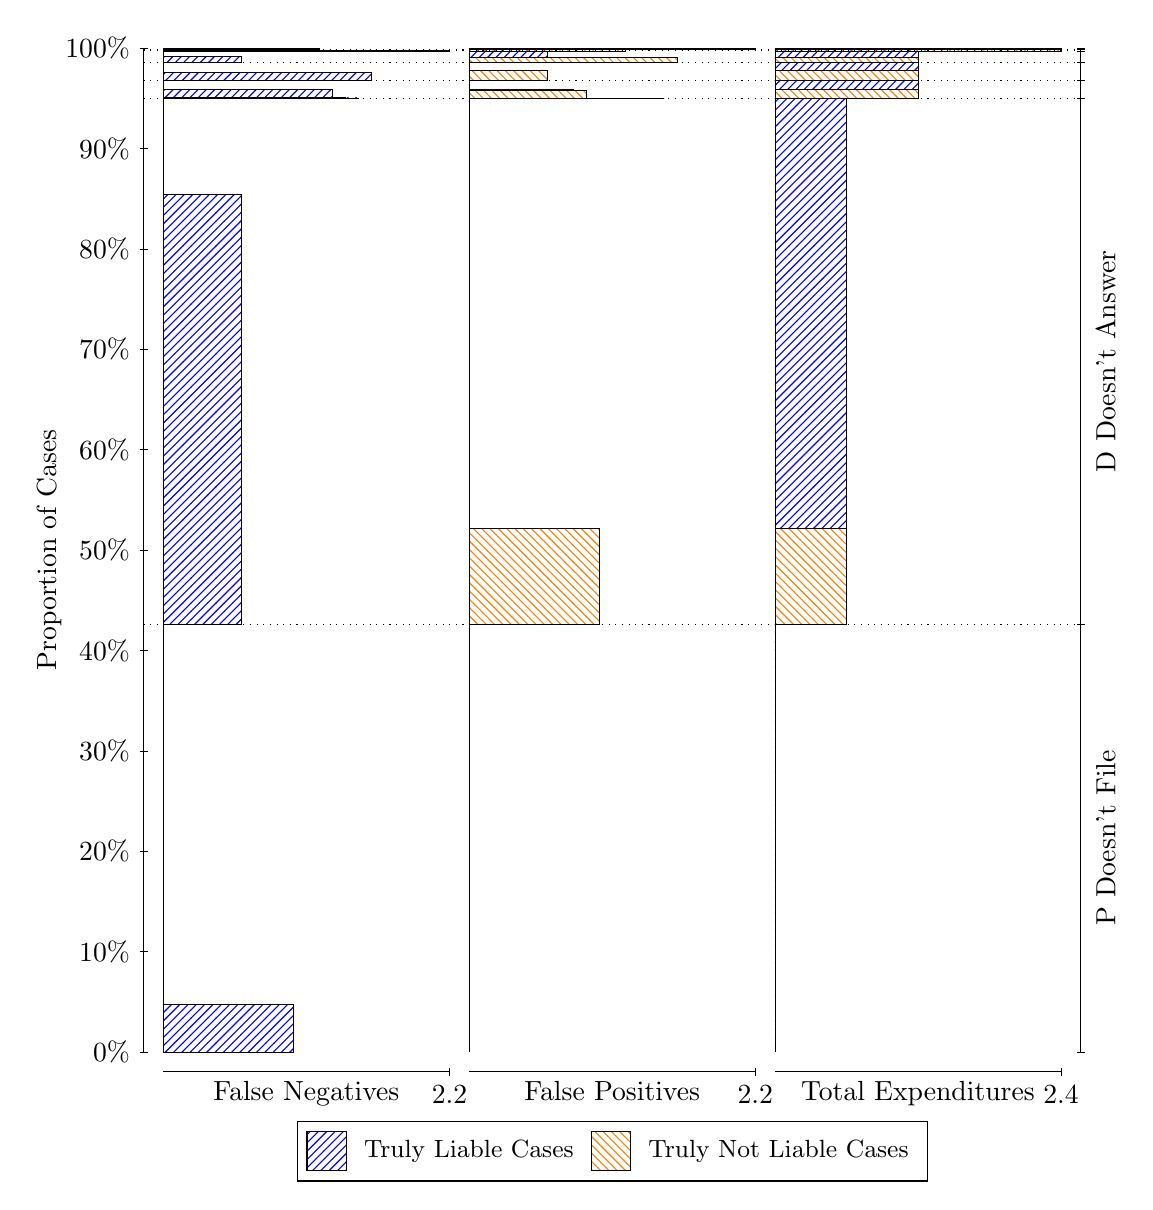
\begin{tikzpicture}
\draw[black, very thin] (1.5,1.75) -- (1.5,14.5);
\node[rotate=90, anchor=center] at (0.3, 8.125) {Proportion of Cases};
\draw[black, very thin] (1.45,1.75) -- (1.55,1.75);
\node[anchor=east] at (1.45, 1.75) {0\%};
\draw[black, very thin] (1.45,3.025) -- (1.55,3.025);
\node[anchor=east] at (1.45, 3.025) {10\%};
\draw[black, very thin] (1.45,4.3) -- (1.55,4.3);
\node[anchor=east] at (1.45, 4.3) {20\%};
\draw[black, very thin] (1.45,5.575) -- (1.55,5.575);
\node[anchor=east] at (1.45, 5.575) {30\%};
\draw[black, very thin] (1.45,6.85) -- (1.55,6.85);
\node[anchor=east] at (1.45, 6.85) {40\%};
\draw[black, very thin] (1.45,8.125) -- (1.55,8.125);
\node[anchor=east] at (1.45, 8.125) {50\%};
\draw[black, very thin] (1.45,9.4) -- (1.55,9.4);
\node[anchor=east] at (1.45, 9.4) {60\%};
\draw[black, very thin] (1.45,10.675) -- (1.55,10.675);
\node[anchor=east] at (1.45, 10.675) {70\%};
\draw[black, very thin] (1.45,11.95) -- (1.55,11.95);
\node[anchor=east] at (1.45, 11.95) {80\%};
\draw[black, very thin] (1.45,13.225) -- (1.55,13.225);
\node[anchor=east] at (1.45, 13.225) {90\%};
\draw[black, very thin] (1.45,14.5) -- (1.55,14.5);
\node[anchor=east] at (1.45, 14.5) {100\%};

\draw[black, very thin] (13.4,1.75) -- (13.4,14.5);
\draw[black, very thin] (13.35,1.75) -- (13.45,1.75);
\node[anchor=west] at (13.35, 1.75) {};
\draw[black, very thin] (13.35,7.1828) -- (13.45,7.1828);
\node[anchor=west] at (13.35, 7.1828) {};
\draw[black, very thin] (13.35,13.862) -- (13.45,13.862);
\node[anchor=west] at (13.35, 13.862) {};
\draw[black, very thin] (13.35,14.092) -- (13.45,14.092);
\node[anchor=west] at (13.35, 14.092) {};
\draw[black, very thin] (13.35,14.314) -- (13.45,14.314);
\node[anchor=west] at (13.35, 14.314) {};
\draw[black, very thin] (13.35,14.465) -- (13.45,14.465);
\node[anchor=west] at (13.35, 14.465) {};
\draw[black, very thin] (13.35,14.485) -- (13.45,14.485);
\node[anchor=west] at (13.35, 14.485) {};
\draw[black, very thin] (13.35,14.5) -- (13.45,14.5);
\node[anchor=west] at (13.35, 14.5) {};

\draw[black, very thin, pattern color=blue, pattern=north east lines] (1.75,1.75) rectangle (3.4015,2.3568);
\draw[black, very thin, pattern color=orange, pattern=north west lines] (1.75,2.3568) rectangle (1.75,7.1828);
\draw[black, very thin, pattern color=blue, pattern=north east lines] (1.75,7.1828) rectangle (2.7409,12.644);
\draw[black, very thin, pattern color=orange, pattern=north west lines] (1.75,12.644) rectangle (1.75,13.862);
\draw[black, very thin, pattern color=blue, pattern=north east lines] (1.75,13.862) rectangle (4.2273,13.868);
\draw[black, very thin, pattern color=blue, pattern=north east lines] (1.75,13.868) rectangle (4.0621,13.876);
\draw[black, very thin, pattern color=blue, pattern=north east lines] (1.75,13.876) rectangle (3.897,13.976);
\draw[black, very thin, pattern color=blue, pattern=north east lines] (1.75,13.976) rectangle (3.7318,13.976);
\draw[black, very thin, pattern color=blue, pattern=north east lines] (1.75,13.976) rectangle (3.5667,13.976);
\draw[black, very thin, pattern color=blue, pattern=north east lines] (1.75,13.976) rectangle (3.4015,13.976);
\draw[black, very thin, pattern color=blue, pattern=north east lines] (1.75,13.976) rectangle (3.2364,13.976);
\draw[black, very thin, pattern color=blue, pattern=north east lines] (1.75,13.976) rectangle (3.0712,13.976);
\draw[black, very thin, pattern color=blue, pattern=north east lines] (1.75,13.976) rectangle (2.9061,13.976);
\draw[black, very thin, pattern color=orange, pattern=north west lines] (1.75,13.976) rectangle (1.75,14.092);
\draw[black, very thin, pattern color=blue, pattern=north east lines] (1.75,14.092) rectangle (4.3924,14.189);
\draw[black, very thin, pattern color=orange, pattern=north west lines] (1.75,14.189) rectangle (1.75,14.314);
\draw[black, very thin, pattern color=blue, pattern=north east lines] (1.75,14.314) rectangle (2.7409,14.394);
\draw[black, very thin, pattern color=orange, pattern=north west lines] (1.75,14.394) rectangle (1.75,14.465);
\draw[black, very thin, pattern color=blue, pattern=north east lines] (1.75,14.465) rectangle (5.3833,14.473);
\draw[black, very thin, pattern color=orange, pattern=north west lines] (1.75,14.473) rectangle (1.75,14.485);
\draw[black, very thin, pattern color=blue, pattern=north east lines] (1.75,14.485) rectangle (3.7318,14.493);
\draw[black, very thin, pattern color=orange, pattern=north west lines] (1.75,14.493) rectangle (1.75,14.5);
\draw[black, very thin, pattern color=orange, pattern=north west lines] (5.6333,1.75) rectangle (5.6333,6.576);
\draw[black, very thin, pattern color=blue, pattern=north east lines] (5.6333,6.576) rectangle (5.6333,7.1828);
\draw[black, very thin, pattern color=orange, pattern=north west lines] (5.6333,7.1828) rectangle (7.2848,8.4012);
\draw[black, very thin, pattern color=blue, pattern=north east lines] (5.6333,8.4012) rectangle (5.6333,13.862);
\draw[black, very thin, pattern color=orange, pattern=north west lines] (5.6333,13.862) rectangle (8.1106,13.862);
\draw[black, very thin, pattern color=orange, pattern=north west lines] (5.6333,13.862) rectangle (7.9455,13.862);
\draw[black, very thin, pattern color=orange, pattern=north west lines] (5.6333,13.862) rectangle (7.7803,13.862);
\draw[black, very thin, pattern color=orange, pattern=north west lines] (5.6333,13.862) rectangle (7.6152,13.862);
\draw[black, very thin, pattern color=orange, pattern=north west lines] (5.6333,13.862) rectangle (7.45,13.862);
\draw[black, very thin, pattern color=orange, pattern=north west lines] (5.6333,13.862) rectangle (7.2848,13.862);
\draw[black, very thin, pattern color=orange, pattern=north west lines] (5.6333,13.862) rectangle (7.1197,13.962);
\draw[black, very thin, pattern color=orange, pattern=north west lines] (5.6333,13.962) rectangle (6.9545,13.97);
\draw[black, very thin, pattern color=orange, pattern=north west lines] (5.6333,13.97) rectangle (6.7894,13.978);
\draw[black, very thin, pattern color=blue, pattern=north east lines] (5.6333,13.978) rectangle (6.4591,13.978);
\draw[black, very thin, pattern color=blue, pattern=north east lines] (5.6333,13.978) rectangle (6.2939,13.978);
\draw[black, very thin, pattern color=blue, pattern=north east lines] (5.6333,13.978) rectangle (6.1288,13.978);
\draw[black, very thin, pattern color=blue, pattern=north east lines] (5.6333,13.978) rectangle (5.9636,13.978);
\draw[black, very thin, pattern color=blue, pattern=north east lines] (5.6333,13.978) rectangle (5.7985,13.978);
\draw[black, very thin, pattern color=blue, pattern=north east lines] (5.6333,13.978) rectangle (5.6333,14.092);
\draw[black, very thin, pattern color=orange, pattern=north west lines] (5.6333,14.092) rectangle (6.6242,14.216);
\draw[black, very thin, pattern color=blue, pattern=north east lines] (5.6333,14.216) rectangle (5.6333,14.314);
\draw[black, very thin, pattern color=orange, pattern=north west lines] (5.6333,14.314) rectangle (8.2758,14.386);
\draw[black, very thin, pattern color=blue, pattern=north east lines] (5.6333,14.386) rectangle (6.6242,14.465);
\draw[black, very thin, pattern color=orange, pattern=north west lines] (5.6333,14.465) rectangle (7.6152,14.478);
\draw[black, very thin, pattern color=blue, pattern=north east lines] (5.6333,14.478) rectangle (5.9636,14.485);
\draw[black, very thin, pattern color=orange, pattern=north west lines] (5.6333,14.485) rectangle (9.2667,14.492);
\draw[black, very thin, pattern color=blue, pattern=north east lines] (5.6333,14.492) rectangle (7.6152,14.5);
\draw[black, very thin, pattern color=orange, pattern=north west lines] (9.5167,1.75) rectangle (9.5167,6.576);
\draw[black, very thin, pattern color=blue, pattern=north east lines] (9.5167,6.576) rectangle (9.5167,7.1828);
\draw[black, very thin, pattern color=orange, pattern=north west lines] (9.5167,7.1828) rectangle (10.425,8.4012);
\draw[black, very thin, pattern color=blue, pattern=north east lines] (9.5167,8.4012) rectangle (10.425,13.862);
\draw[black, very thin, pattern color=orange, pattern=north west lines] (9.5167,13.862) rectangle (11.333,13.862);
\draw[black, very thin, pattern color=blue, pattern=north east lines] (9.5167,13.862) rectangle (11.333,13.862);
\draw[black, very thin, pattern color=orange, pattern=north west lines] (9.5167,13.862) rectangle (11.333,13.978);
\draw[black, very thin, pattern color=blue, pattern=north east lines] (9.5167,13.978) rectangle (11.333,14.092);
\draw[black, very thin, pattern color=orange, pattern=north west lines] (9.5167,14.092) rectangle (11.333,14.092);
\draw[black, very thin, pattern color=blue, pattern=north east lines] (9.5167,14.092) rectangle (11.333,14.092);
\draw[black, very thin, pattern color=orange, pattern=north west lines] (9.5167,14.092) rectangle (11.333,14.216);
\draw[black, very thin, pattern color=blue, pattern=north east lines] (9.5167,14.216) rectangle (11.333,14.314);
\draw[black, very thin, pattern color=orange, pattern=north west lines] (9.5167,14.314) rectangle (11.333,14.386);
\draw[black, very thin, pattern color=blue, pattern=north east lines] (9.5167,14.386) rectangle (11.333,14.465);
\draw[black, very thin, pattern color=orange, pattern=north west lines] (9.5167,14.465) rectangle (13.15,14.478);
\draw[black, very thin, pattern color=blue, pattern=north east lines] (9.5167,14.478) rectangle (13.15,14.485);
\draw[black, very thin, pattern color=orange, pattern=north west lines] (9.5167,14.485) rectangle (13.15,14.492);
\draw[black, very thin, pattern color=blue, pattern=north east lines] (9.5167,14.492) rectangle (13.15,14.5);
\draw[black, dotted] (1.5,7.1828) -- (13.4,7.1828);
\draw[black, dotted] (1.5,13.862) -- (13.4,13.862);
\draw[black, dotted] (1.5,14.092) -- (13.4,14.092);
\draw[black, dotted] (1.5,14.314) -- (13.4,14.314);
\draw[black, dotted] (1.5,14.465) -- (13.4,14.465);
\draw[black, dotted] (1.5,14.485) -- (13.4,14.485);
\draw[black, very thin] (1.75,1.5) -- (5.3833,1.5);
\node[anchor=north] at (3.5667, 1.5) {False Negatives};
\draw[black, very thin] (5.3833,1.45) -- (5.3833,1.55);
\node[anchor=north] at (5.3833, 1.45) {2.2};

\draw[black, very thin] (5.6333,1.5) -- (9.2667,1.5);
\node[anchor=north] at (7.45, 1.5) {False Positives};
\draw[black, very thin] (9.2667,1.45) -- (9.2667,1.55);
\node[anchor=north] at (9.2667, 1.45) {2.2};

\draw[black, very thin] (9.5167,1.5) -- (13.15,1.5);
\node[anchor=north] at (11.333, 1.5) {Total Expenditures};
\draw[black, very thin] (13.15,1.45) -- (13.15,1.55);
\node[anchor=north] at (13.15, 1.45) {2.4};

\node[black, centered, rotate=90] at (13.72, 4.4664) {P Doesn't File};
\node[black, centered, rotate=90] at (13.72, 10.522) {D Doesn't Answer};






\draw (7.449999999999999,1.5) node[draw=none] (baseCoordinate) {};
\begin{scope}[align=center]
        \matrix[scale=0.5, draw=black, below=0.5cm of baseCoordinate, nodes={draw}, column sep=0.1cm]{
            \node[rectangle, draw, minimum width=0.5cm, minimum height=0.5cm, pattern=north east lines, pattern color=blue] {}; &
            \node[draw=none, font=\small] (B) {Truly Liable Cases}; &
            \node[rectangle, draw, minimum width=0.5cm, minimum height=0.5cm, pattern=north west lines, pattern color=orange] {}; &
            \node[draw=none, font=\small] (B) {Truly Not Liable Cases}; \\
            };
\end{scope}

\end{tikzpicture}
\end{document}